\documentclass[a4paper]{ltxguide}
\usepackage[utf8]{inputenc}
\usepackage[frenchb]{babel}
\usepackage{graphicx}
\usepackage{caption}
\renewcommand{\familydefault}{\sfdefault}
\title{User Guide of Obigo}
\author{Vincent Ferreira and Adrien Guille}
\date{\today}
\begin{document}

\maketitle
\tableofcontents

\section{Requirements}

Java SDK installed (at least 1.5).

\section{Installation}

The game is nested in a jar file.
Make the jar file by executing (from the command shell) :

\begin{center}
\texttt{mvn package}
\end{center}
Then run the installer by executing (from the command shell) :

\begin{center}
\texttt{java -jar target/Obi-Go-1.0.jar}
\end{center}
\section{Playing Instructions}

\begin{center}
	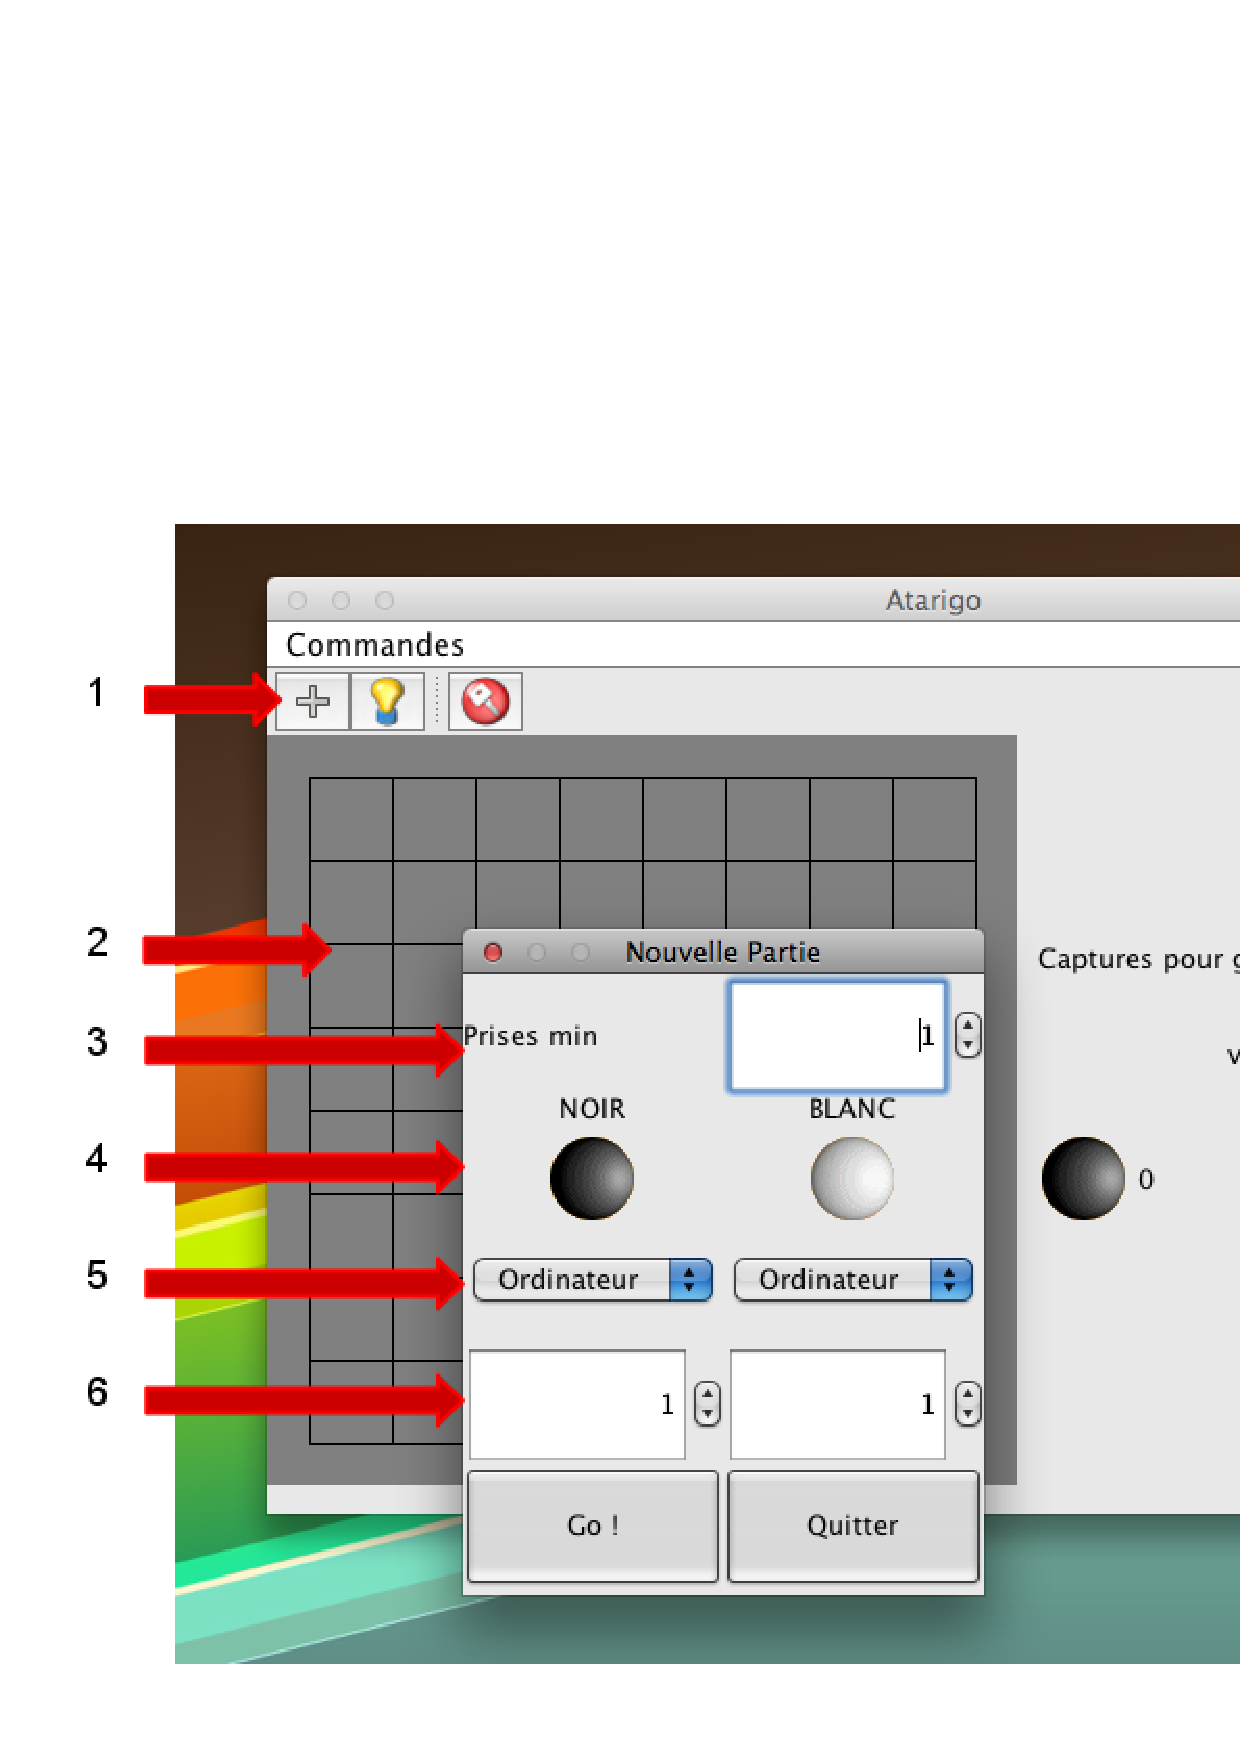
\includegraphics[scale=0.50]{images/capture}
	\captionof{figure}{Screenshot of the captioned user interface}
\end{center}

\Paragraph\textbf{\underline{Start the game}}

To start the game you have to click on the little cross up in the tool bar. A window will open giving you access to the parameters of your game. We present you down here a description of the different parameters of the game :

\begin{itemize}
\item\textbf{Minimal captures (3) :}  It's  the amount of minimum captures that a player must do to win. By default this number is initialised at 1 to fit to the originals rules of Atarigo.

\item\textbf{Type of player (5) :} Here, we choose if the player fitting to the color (4) is a human or an AI. The black always make the first move. We can play every type of game, including AI vs AI.

\item\textbf{Depth of the minimax search (6) :} If the player is an AI type, thi number will be the depth gone through by the AI. Increasing this number also mean an increase of a difficulty for a human opponent. The value of 1 corresponds to a fast thinking time. The value of 4 will ask a longer thinking time of many seconds.
\end{itemize}

	Once the parameters established , click on the «Go!» button to start the game. To put a stone on the board, you need to click on the wished place. A ghost position is given to see where the stone will be put. When you made your move, the turn is given to the other player. If this player is an AI, the stone is put automatically. It's possible you have to wait before the AI end his turn.

	You can see right to the board some informations about the current game. From the top these informations are :

	\begin{itemize}
	\item{The amount of minimale captures to win.}

	\item{The left captures by players.}

	\item{The depth of the minimax search if the player is an AI.}
	\end{itemize}

    The game is over when a player made all the captures required or when a player can't make a move. You can start a new game whenever you want which will end the current game you where playing.


\Paragraph\textbf{\underline{Quit the application}}

    To quit the application, click on the cross of the application windows or on the key icon in the tool bar.

\section{Use tips}

    If you play against an high AI, it's disadvised to click on the board during his time of thinking.


\end{document}
